\lipsum[1]

\begin{table}[!htb]
  \centering
  \resizebox{0.485\textwidth}{!}{%  % This line changes the table width
    \begin{tabular}{|c|l|c|c|}
      \hline
      \multicolumn{4}{|c|}{\textbf{Parametros}}                                    \\
      \hline
      \textbf{Functions} & \textbf{Parameters} & \textbf{Results} & \textbf{Error} \\
      \hline
      \multirow{5}{*}{Coffee}
                         & Roast Level         & \(Dark\)         & \(N/A\)        \\
                         & Caffeine (mg)       & \(90\)           & \(5\)          \\
                         & Volume (ml)         & \(350\)          & \(10\)         \\
                         & Temperature (ºC)    & \(80\)           & \(2\)          \\
                         & Milk Volume (ml)    & \(50\)           & \(5\)          \\
      \hline
      \multirow{4}{*}{Pizza}
                         & Diameter (cm)       & \(30\)           & \(1\)          \\
                         & Toppings            & \(Pepperoni\)    & \(N/A\)        \\
                         & Calories            & \(2000\)         & \(100\)        \\
                         & Slices              & \(8\)            & \(0\)          \\
      \hline
    \end{tabular}
  }
  \caption{An example table with one column width.}
\end{table}

\lipsum[1]

\begin{table*}[h!]
  \centering
  \begin{tabular}{|c|l|c|c|}
    \hline
    \multicolumn{4}{|c|}{\textbf{The Ultimate Caffeine + Junk Food Smackdown}}                                     \\
    \hline
    \textbf{Beverages/Snacks} & \textbf{Parameters}         & \textbf{Epic Results} & \textbf{Confidence Interval} \\
    \hline
    \multirow{5}{*}{Espresso Extravaganza}
                              & Brew Time (seconds)         & \(30\)                & \(1\)                        \\
                              & Jitters Factor (\%)         & \(120\)               & \(±5\)                       \\
                              & Hipster Approval Rating     & \(100\)               & \(N/A\)                      \\
                              & Ideal Sipping Temp (ºC)     & \(85\)                & \(2\)                        \\
                              & Existential Crises Averted  & \(7\)                 & \(±1\)                       \\
    \hline
    \multirow{5}{*}{Donut Delirium}
                              & Sugar Coma Threshold (mins) & \(15\)                & \(3\)                        \\
                              & Sprinkle Count              & \(Hundreds, maybe?\)  & \(Don't make me count!\)     \\
                              & Glaze Viscosity (cP)        & \(500\)               & \(50\)                       \\
                              & 'Dunkability' Score         & \(9.5/10\)            & \(±0.2\)                     \\
                              & Eaten By (team members)     & \(Everyone\)          & \(N/A\)                      \\
    \hline
  \end{tabular}
  \caption{A stupid full-width table generated with GPT.}
\end{table*}

\lipsum[1-5]

\lipsum[1-4]

\begin{figure*}[h!]
  \centering
  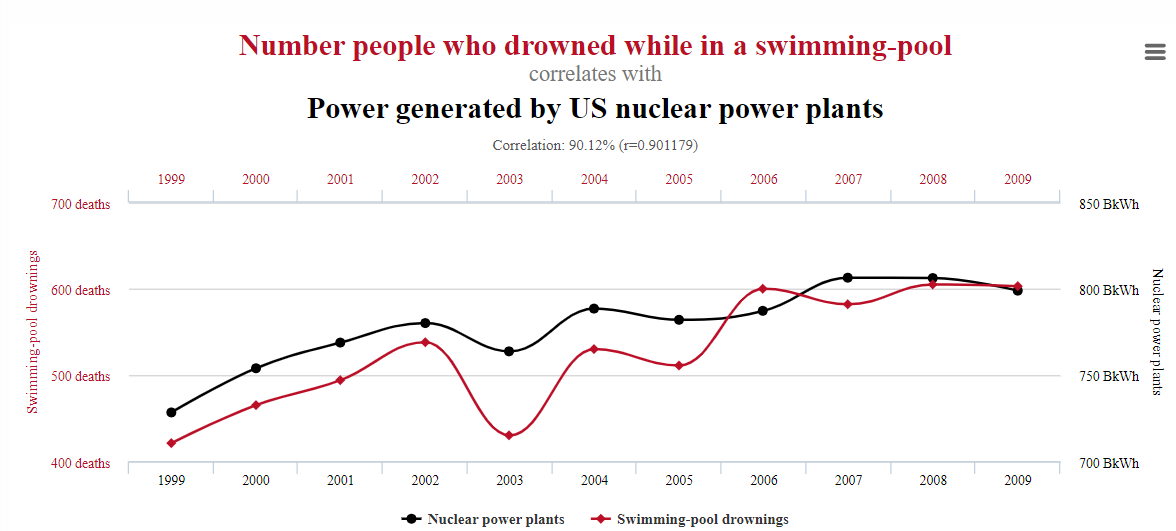
\includegraphics[width=\textwidth]{images/correlation.png}
  \caption{An example of figure spanning two columns.}
  \label{fig:your_label}
\end{figure*}


\lipsum[1-4]